%!TEX root = book.tex
\section{Emergency Stress Test}

\setSpacing{1.5}
\subsection{Problem Statement}

องค์การบริการกู้ภัยฉุกเฉิน (Emergency Response Service Authority; ERSA) กำลังจะจัดงานซ้อมทดสอบกู้ภัยประจำปี ซึ่งจัดขึ้น ณ ถนนทางหลวงทางตรงสายหนึ่ง เพื่อทดสอบขีดความสามารถในการตอบสนองต่อภัยที่เกิดขึ้นที่อาจเกิดขึ้นอย่างฉับพลันและพร้อมกันในหลาย\,ๆ จุด \;
สมาชิกหน่วยกู้ภัยฉุกเฉินแต่ละคนจากทั้งหมด \lstinline{n} คนจะประจำการอยู่ที่จุดต่าง\,ๆ บนทางหลวงสายนี้ \;
ทางหลวงสายนี้เปรียบเสมือนเส้นจำนวนในแกน X และจุดต่าง\,ๆ บนทางหลวงสามารถแทนได้ด้วยพิกัดบนแกน X \;
นอกจากนี้ระยะทาง 1 เมตรบนทางหลวงสายนี้มีค่าเท่ากับระยะ 1 หน่วยบนแกน X

การทดสอบจะเริ่มขึ้นเมื่อมีเสียงนกหวีด \;\;
เมื่อเสียงนกหวีดดังขึ้น นาฬิกาจับเวลา \lstinline{m} เรือนจะปรากฏขึ้นตามสถานที่ตำแหน่งต่าง\,ๆ บนทางหลวง \;
นอกจากนั้นนาฬิกาแต่ละเรือนจะเริ่มนับเวลาถอยหลังจากค่าเริ่มต้นที่แตกต่างกัน \;
เป้าหมายของทีมหน่วยกู้ภัยโดยรวมคือจะต้องส่งสมาชิกของทีมตัวเองไปเคลมนาฬิกาจับเวลาให้ได้จำนวนมากที่สุดก่อนนาฬิกาเรือนนั้น\,ๆ หมดเวลาลงเสียก่อน \;
ตลอดเวลาที่ทำการทดสอบนี้ สมาชิกทีมกู้ภัยแต่ละคนสามารถเคลมนาฬิกาได้อย่างมากที่สุด 1 เรือน และนาฬิกาเรือนดังกล่าวจะถูกเคลมได้หากสมาชิกคนนั้นวิ่งไปถึงนาฬิกาเรือนดังกล่าวก่อนหมดเวลาหรือทันเวลาฉิวเฉียดพอดีเท่านั้น

หมายเหตุ กฎความปลอดภัยของทีมหน่วยกู้ภัยคือ สมาชิกแต่ละคนสามารถเคลื่อนไหวด้วยอัตราเร็วสูงสุด 1 เมตรต่อวินาทีเท่านั้น


\setSpacing{1.5}
\subsection{Situation Example}

ลองพิจารณาตัวอย่างสถานการณ์ดังนี้ \;
สมมติว่า ทีมหน่วยกู้ภัยมีสมาชิกทั้งสิ้น 
\lstinline{n} \lstinline{=} \lstinline{3} คน 
แต่ละคนประจำการอยู่ที่ตำแหน่ง
\lstinline{x} \lstinline{=} \lstinline{1}, 
\lstinline{x} \lstinline{=} \lstinline{3} 
และ \lstinline{x} \lstinline{=} \lstinline{5} ตามลำดับ

เมื่อเสียงนกหวีดดังขึ้น นาฬิกาจับเวลา \lstinline{m = 5} เรือนปรากฏขึ้นดังต่อไปนี้
\begin{itemize}[leftmargin=4pc]
    \item  นาฬิกาเรือนที่ 1 ปรากฏที่ตำแหน่ง \lstinline{x = -6} และเริ่มต้นนับเวลาถอยหลังที่ \lstinline{7} วินาที
    \item  นาฬิกาเรือนที่ 2 ปรากฏที่ตำแหน่ง \lstinline{x = 10} และเริ่มต้นนับเวลาถอยหลังที่ \lstinline{6} วินาที
    \item  นาฬิกาเรือนที่ 3 ปรากฏที่ตำแหน่ง \lstinline{x = 11} และเริ่มต้นนับเวลาถอยหลังที่ \lstinline{3} วินาที
    \item  นาฬิกาเรือนที่ 4 ปรากฏที่ตำแหน่ง \lstinline{x = -2} และเริ่มต้นนับเวลาถอยหลังที่ \lstinline{2} วินาที
    \item  นาฬิกาเรือนที่ 5 ปรากฏที่ตำแหน่ง \lstinline{x = -4} และเริ่มต้นนับเวลาถอยหลังที่ \lstinline{5} วินาที
\end{itemize}

\begin{center}
    \bigskip
    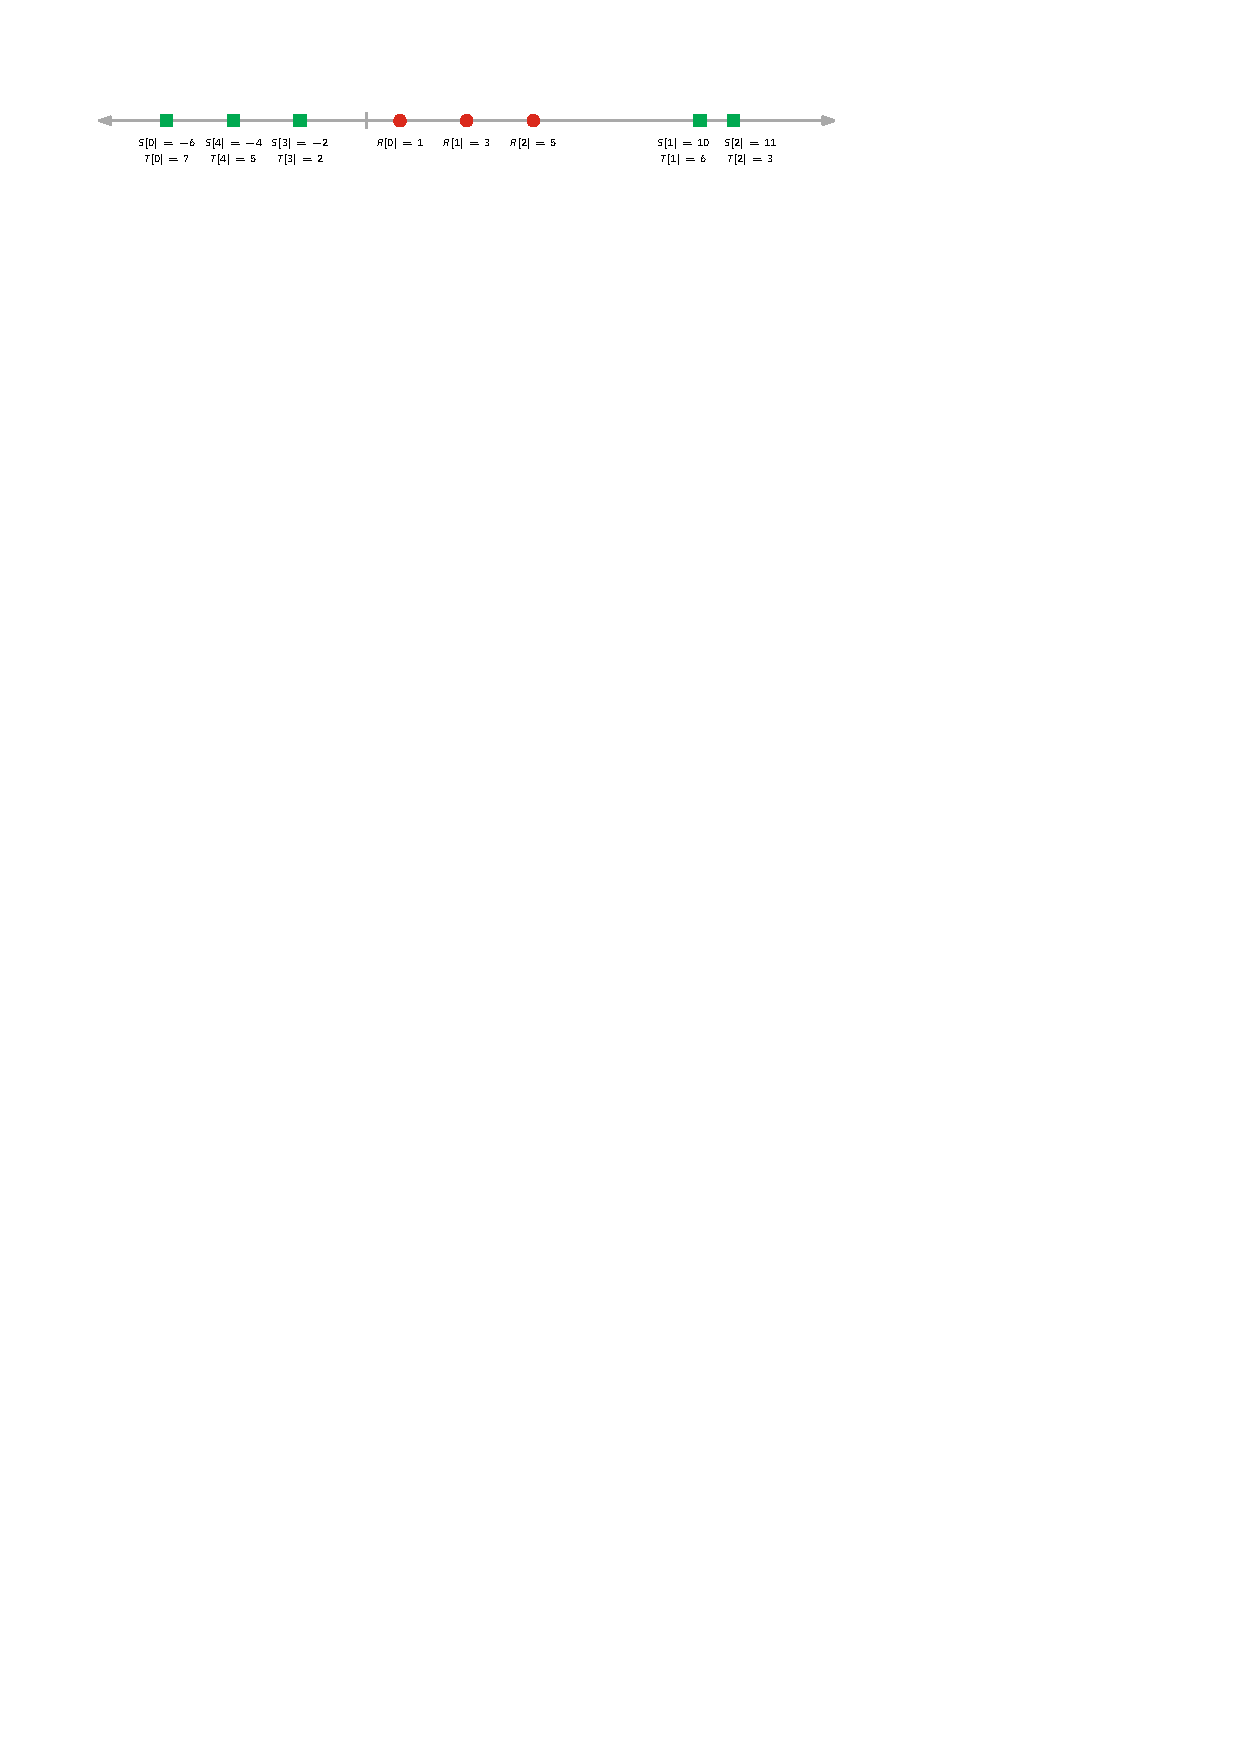
\includegraphics[page=1,scale=1.2]{figures/est.pdf}
    \smallskip
\end{center}

ในกรณีนี้ ทีมหน่วยกู้ภัยจะสามารถเคลมนาฬิกาจับเวลาได้มากที่สุดเพียง 2 เรือนเท่านั้น นั่นคือ
\begin{itemize}[leftmargin=4pc]
    \item  สมาชิกที่ประจำอยู่ที่ตำแหน่ง \lstinline{x = 1} เคลมนาฬิกาเรือนที่ 1 อย่างทันฉิวเฉียด
    \item  สมาชิกที่ประจำอยู่ที่ตำแหน่ง \lstinline{x = 5} เคลมนาฬิกาเรือนที่ 2 ก่อนหมดเวลา 1 วินาทีพอดี
\end{itemize}


\setSpacing{1.5}
\subsection{Objectives}

\noindent
จงเขียนโปรแกรมเพื่อรับ Input Data ต่อไปนี้

\begin{itemize}
    \item
        ข้อมูลเกี่ยวกับสมาชิกทีมหน่วยกู้ภัยทั้งสิ้น \lstinline{n} ราย\: (โดยที่ \lstinline{1 ≤ n ≤ 200,000}) \\
        กล่าวคือสมาชิกกู้ภัยคนที่ \lstinline{i} สำหรับ \lstinline{i} \lstinline{=} \lstinline{0}, \lstinline{1}, \ldots, \lstinline{n-1} จะมีข้อมูลดังต่อไปนี้
        \begin{itemize}
            \item \lstinline{R[i]} คือตำแหน่งเริ่มต้นบนแกน X ของสมาชิกคนที่ \lstinline{i} \\
            (โดยที่ \lstinline{-1,000,000,000 ≤ R[i] ≤ 1,000,000,000})
        \end{itemize}
    \item
        ข้อมูลของนาฬิกาทั้งสิ้น \lstinline{m} เรือนที่ปรากฏขึ้นเมื่อเริ่มเสียงสัญญาณนกหวีด\: (โดยที่ \lstinline{1 ≤ m ≤ 200,000}) \\
        กล่าวคือนาฬิกาเรือนที่ \lstinline{j} สำหรับ \lstinline{j} \lstinline{=} \lstinline{0}, \lstinline{1}, \ldots, \lstinline{m-1} จะมีข้อมูลดังต่อไปนี้
        \begin{itemize}
            \item  \lstinline{S[j]} คือตำแหน่งที่นาฬิกาเรือนที่ \lstinline{j} ปรากฏบนแกน X \\
            (โดยที่ \lstinline{-1,000,000,000 ≤ S[j] ≤ 1,000,000,000})
            \item \lstinline{T[j]} คือเวลาเริ่มต้นของนาฬิกาเรือนที่ \lstinline{j} ในหน่วยวินาที \\
            (โดยที่ \lstinline{0 ≤ T[j] ≤ 1,000,000,000})
        \end{itemize}
\end{itemize}

\noindent
แล้วจึงคำนวณ\uline{จำนวนนาฬิกาที่สามารถเคลมได้มากที่สุดเท่าที่เป็นไปได้} และคืนค่าคำตอบดังกล่าวเป็น Output Data ของโปรแกรม


\setSpacing{1.5}
\subsection{Interfaces and Data Format}

\noindent
โปรแกรมที่เขียนขึ้นจะต้องรับ Input Data ผ่าน Standard Input ซึ่งมีรูปแบบดังต่อไปนี้

\begin{itemize}[topsep=0pc,itemsep=0pt]
    \item
        บรรทัดแรกมีจำนวนเต็มสองจำนวน \lstinline{n} และ \lstinline{m}
    \item 
        บรรทัดที่ \lstinline{i+2} 
        สำหรับ \lstinline{i} \lstinline{=} \lstinline{0}, \lstinline{1}, \ldots, \lstinline{n-1}
        จะมีจำนวนเต็มหนึ่งจำนวน ซึ่งก็คือ \lstinline{R[i]}
    \item 
        บรรทัดที่ \lstinline{n+j+2}
        สำหรับ \lstinline{j} \lstinline{=} \lstinline{0}, \lstinline{1}, \ldots, \lstinline{m-1}
        จะมีจำนวนเต็มสองจำนวนที่ถูกคั่นด้วยช่องว่าง \\
        ซึ่งก็คือ \lstinline{S[j]} และ \lstinline{T[j]}
\end{itemize}

\begin{lstlisting}[aboveskip=1pc,xleftmargin=6pc]
n m
R[0]
R[1]            <%\SuppressNumber\AlternateNumber{...}%>
                <%\AlternateNumber{n+1}%>
R[n-1]          <%\AlternateNumber{n+2}%>
S[0] T[0]       <%\AlternateNumber{n+3}%>
S[1] T[1]       <%\AlternateNumber{...}%>
                <%\AlternateNumber{n+m+1}%>
S[m-1] T[m-1]   <%\ReactivateNumber%>
\end{lstlisting}

\noindent
โปรแกรมที่เขียนขึ้นจะต้องคืน Output Data ผ่าน Standard Output เป็นจำนวนเต็ม 1 จำนวน ซึ่งเป็นคำตอบของโจทย์ตามที่ระบุไว้ในหัวข้อ Objectives ข้างต้น

\newpage
\begin{center}
\smallskip\small
\begin{tabular}{p{0.425\linewidth}p{0.425\linewidth}}
\toprule
Example Input & Example Output \\
\midrule
\ttfamily\setSpacing{1}
3 5 \newline
1 \newline
3 \newline
5 \newline
-6 7 \newline
10 6 \newline
11 3 \newline
-2 2 \newline
-4 5 &
\ttfamily\setSpacing{1}
2 \\
\bottomrule
\end{tabular}
\end{center}


\setSpacing{1.5}
\subsection{Scoring}

\noindent
โปรแกรมของคุณจะถูกทดสอบกับ Test Cases ที่มีเงื่อนไขต่าง\,ๆ ดังนี้

\begin{description}
    \item[SMALL] (คะแนน 20\%) \\
        รับประกันว่าจำนวนของสมาชิกกู้ภัยและจำนวนของนาฬิกาจะสอดคล้องกับเงื่อนไข \lstinline{1 ≤ n,m ≤ 1,000} และค่าพิกัดแกน X จะอยู่ในช่วงตั้งแต่ \lstinline{-100,000} จนถึง \lstinline{100,000}
    \item[MEDIUM] (คะแนน 35\%) \\
        รับประกันว่าค่าพิกัดแกน X จะอยู่ในช่วงตั้งแต่ \lstinline{-100,000} จนถึง \lstinline{100,000}
    \item[LARGE] (คะแนน 45\%) \\
        ไม่มีเงื่อนไขเพิ่มเติม
\end{description}


\setSpacing{1.5}
\subsection{Limitations}

\noindent
โปรแกรมจะถูกจำกัดเวลาอยู่ที่ 1.0 วินาทีต่อ Test Case (baseline) และถูกจำกัดหน่วยความจำอยู่ที่ 512 MB
\begin{itemize}
    \item 
        สำหรับโปรแกรมที่เขียนด้วยภาษา C หรือ C++ จะถูกจำกัดเวลาเท่ากับค่า baseline ข้างต้น
    \item 
        สำหรับโปรแกรมที่เขียนด้วยภาษา Go หรือ Java จะถูกจำกัดเวลาอยู่ที่ 1.5 เท่าของ baseline ข้างต้น
    \item 
        สำหรับโปรแกรมที่เขียนด้วยภาษา JavaScript หรือ Python จะถูกจำกัดเวลาอยู่ที่ 2.5 เท่าของ baseline ข้างต้น
\end{itemize}
